\documentclass[11pt,a4paper]{article}

\usepackage[utf8]{inputenc}
\usepackage[T1]{fontenc}
\usepackage[margin=2.5cm]{geometry}
\usepackage{booktabs}
\usepackage{graphicx}
\usepackage{amsmath}
\usepackage{caption}
\usepackage[hidelinks]{hyperref}
\usepackage{xcolor}

\title{A Joint Embedding Predictive World Model for JAXAtari\\
\large Implementing and evaluating LeWorldModel on the JAXAtari-15 suite}
\author{Amirmohammad Raei\\
Praktikum in der KI, Topic 30 (Deep model based RL: JEPA and Dreamer)\\
Technische Universit\"at Darmstadt}
\date{September 2026}

\begin{document}
\maketitle

\begin{abstract}
This report describes an implementation of LeWorldModel (LeWM), a joint embedding
predictive architecture for learning world models directly from pixels, and its
evaluation on the fifteen games of the JAXAtari suite. No JAX or JAXAtari
implementation of the method existed, so the model, the training loop, the
evaluation protocol and the downstream agent were all written from scratch for
this lab. The world model trains without representation collapse on all fifteen
games and produces useful open loop latent predictions on fourteen of them. A set
of seven single variable ablations tests the paper's central architectural claim,
that the SIGReg regulariser removes the need for a stop gradient. The claim is
partly supported and partly narrowed: removing SIGReg does collapse the
representation, but a plain stop gradient also prevents collapse, so SIGReg is
sufficient rather than necessary, and what it actually contributes is a
substantially better predictor. Finally, a PPO agent is trained on the frozen
representation and compared against an identical agent trained from raw pixels.
Averaged over three seeds on Pong, the pretrained representation roughly halves
the number of environment steps needed to reach positive play and reduces run to
run variance by a factor of about seven, while the final score after one million
steps is not significantly different.
\end{abstract}

\section{Introduction}

Model based reinforcement learning agents learn a model of the environment and use
it to plan or to shape a policy. Most such models predict future observations in
pixel space, which forces the model to spend capacity on visual detail that is
irrelevant to control. Joint embedding predictive architectures (JEPAs) take a
different route. They predict the \emph{embedding} of a future observation rather
than the observation itself, so that anything the encoder chooses to discard is
also removed from the prediction target.

That design has a well known failure mode. If the encoder is free to choose the
target, it can drive the prediction loss to zero by mapping every input to the
same constant vector. The representation then carries no information at all while
the training loss looks excellent. Methods in this family therefore need some
mechanism that prevents collapse. BYOL and its descendants use a stop gradient on
the target branch together with an exponential moving average target encoder.

LeWorldModel (LeWM) proposes an alternative. It adds a distributional regulariser
called SIGReg, a sketched isotropic Gaussian regulariser, and claims that this term
alone is enough to keep the representation open, so that the whole system can be
trained end to end with no stop gradient and no separate target network. That
claim is architecturally interesting because it simplifies the training setup
considerably, and it is the claim this report sets out to test on a new domain.

The task for this lab was to implement the algorithm on JAXAtari, make it run on
the fifteen required games, and compare the results against existing
implementations. Since the method predicts embeddings and never predicts reward,
it produces no game scores by itself, so an additional downstream evaluation was
built in order to obtain numbers that can be compared with published reinforcement
learning baselines.

\section{Background}

\subsection{The objective}

Let $f_\theta$ be an encoder mapping a single frame to an embedding, and let
$g_\phi$ be a predictor that maps a sequence of embeddings and the actions taken
to a prediction of the next embedding. Writing $z_t = f_\theta(x_t)$, the training
objective is

\begin{equation}
\mathcal{L} = \underbrace{\frac{1}{T}\sum_t \left\| g_\phi(z_{1:t}, a_{1:t}) - z_{t+1} \right\|^2}_{\text{prediction}}
\; + \; \lambda \cdot \underbrace{\mathrm{SIGReg}(z)}_{\text{anti collapse}} .
\end{equation}

The important detail is that the target $z_{t+1}$ is produced by the \emph{same}
encoder, and gradients flow through it. There is no stop gradient and no target
network. Collapse is prevented only by the second term.

\subsection{SIGReg}

SIGReg measures how far the distribution of embeddings is from an isotropic
Gaussian. It draws a large number of random one dimensional projections of the
embedding batch and applies an Epps and Pulley style normality test to each
projection, comparing the empirical characteristic function of the projected data
against that of a standard normal. The statistic is averaged over projections.
Because an isotropic Gaussian occupies all directions of the embedding space
equally, minimising this term directly opposes the concentration of embeddings
into a low dimensional subspace, which is what collapse looks like geometrically.

The implementation of this term follows the reference code of the paper closely,
since it is the component the paper's contribution rests on and any deviation
would make the ablation meaningless.

\section{Implementation}

The whole system is written in PyTorch, with the environment remaining in JAX. The
world model itself is one self contained file of roughly eight hundred lines. The
remaining files are experiment runners, the downstream agent, and tests.

\subsection{Architecture}

\paragraph{Encoder.} Three convolutional layers in the standard Nature DQN
configuration, followed by a linear projection to 256 dimensions and a batch
normalisation layer. The encoder sees a single RGB frame resized to $84 \times 84$.

\paragraph{Predictor.} A four layer causal transformer over the sequence of frame
embeddings. Actions enter through adaptive layer normalisation with a zero
initialised modulation head, as in the paper. Each action produces per token shift,
scale and gate parameters for both sub layers of the block. Because the modulation
head is initialised to zero, every gate starts at zero and the entire predictor is
exactly the identity function at initialisation. The predictor therefore begins as
a no operation and learns to use actions, rather than injecting randomly scaled
action noise into the residual stream from the first step. The output passes
through a projector matching the encoder's, a linear layer followed by batch
normalisation.

\paragraph{Loss.} Mean squared error between predicted and target embeddings, plus
$\lambda = 0.1$ times the SIGReg term, with gradients flowing through the targets.

\subsection{Deviations from the paper}

Three deviations were made, all deliberate and all argued here rather than hidden.

First, the encoder is a convolutional network rather than a vision transformer.
Atari frames are small and visually simple, a convolutional trunk is considerably
cheaper on the hardware available, and the paper itself reports that the method is
encoder agnostic. This is the deviation most likely to matter and it is the one
that would be reverted first if more compute were available.

Second, data is collected online from a uniform random policy rather than from a
prepared offline reward free dataset. The lab provides environments, not datasets,
so an online collector was the natural choice. The consequence is that the model
only ever observes the part of the state space a random agent reaches, which is a
severe restriction on games with sparse rewards such as Montezuma's Revenge.

Third, and most significantly, the trained predictor is never used for control.
The paper evaluates LeWM through model predictive control in the latent space. In
this work the predictor is trained and evaluated as a predictor, and the
downstream agent learns a policy on top of the encoder instead. Latent planning
was not implemented and is the clearest piece of unfinished work.

\subsection{Data collection}

Episodes are played under a uniform random policy and cut into non overlapping
windows of seventeen frames, sixteen for context and one as the final target.
Windows never straddle an episode boundary. Episodes run for up to five hundred
environment steps and the windows kept from a long episode are sampled uniformly
across it rather than taken from the front, so that coverage is not restricted to
the opening seconds of a game. Section~\ref{sec:confounds} explains why this
matters and how the earlier version of the collector was wrong.

\section{Experimental setup}

All experiments in this report were run on a single laptop. The relevant details
are given in Table~\ref{tab:system}, since the lab guidelines ask for information
about the training system.

\begin{table}[h]
\centering
\caption{Hardware and software used for all reported results.}
\label{tab:system}
\begin{tabular}{ll}
\toprule
Machine & Apple M5, 32 GB unified memory \\
Python & 3.11.16 \\
PyTorch & 2.12.0, running on the Metal (MPS) backend \\
JAX & 0.10.1, running on CPU \\
\bottomrule
\end{tabular}
\end{table}

One property of this setup shaped the entire software design and is worth stating
explicitly. JAX has no GPU backend on Apple silicon and therefore runs on CPU,
while PyTorch reaches the GPU through Metal. A benchmark of the Nature CNN trunk at
batch size 512 measured one forward and backward pass at 772 milliseconds under
JAX on CPU against 37 milliseconds under PyTorch on Metal, a factor of roughly
twenty on the operation that dominates policy optimisation. The agent was
originally written in JAX and ran at eight environment steps per second. Rewriting
the networks in PyTorch while leaving the environment in JAX raised this to
roughly 1300 steps per second. This is a property of the hardware rather than of
either framework, and on a CUDA machine the natural choice would be different.

World model training uses 5000 gradient steps per game, a replay buffer that grows
from 600 to 2600 sequences, and the Adam optimiser at a learning rate of
$3 \times 10^{-4}$. Agents are trained for one million environment steps with
hyperparameters matching the repository's own PPO configuration, so that the
comparison against the repository baseline is meaningful.

\section{Evaluating a world model that predicts embeddings}
\label{sec:eval}

Before presenting results, the evaluation protocol needs justification, because the
obvious metric is actively misleading here.

\paragraph{The training loss cannot be trusted.} A collapsed encoder achieves a
\emph{lower} prediction loss than a healthy one, because predicting a constant is
trivial. Any evaluation that reads the loss curve and concludes that training went
well will therefore rate a completely useless model as the best one. This is not a
hypothetical concern. It is exactly what the ablation in
Section~\ref{sec:ablations} demonstrates.

Two diagnostics are used instead.

\paragraph{Effective rank.} The entropy based effective rank of the matrix of
embeddings, out of a maximum of 256. This is the correct collapse metric for this
architecture specifically because the encoder ends in batch normalisation, which
pins the variance of every individual dimension to one. Collapse therefore cannot
show up as shrinking embedding norms, which is the naive thing to measure. It shows
up as the embeddings occupying a low dimensional subspace, and that is what
effective rank detects. A value near one means total collapse.

\paragraph{Open loop rollout error against a trivial baseline.} The predictor is
given three true embeddings and then run autoregressively on its own outputs for
fourteen further steps. The resulting mean squared error is compared against a
trivial predictor that simply assumes the embedding never changes. Because mean
squared error in a learned latent space has no absolute scale, and because
different training configurations produce differently scaled latent spaces, only
the ratio between the model and its own baseline is comparable across
configurations. All rollout numbers in this report are therefore reported as that
ratio, where a value of one means no better than assuming nothing happens.

\section{World model results}

\begin{table}[h]
\centering
\caption{World model after 5000 training steps on each of the fifteen required
games. The ratio column is open loop rollout error divided by that model's own
frozen baseline, so lower is better and 1.0 means no better than assuming the
embedding never changes.}
\label{tab:games}
\begin{tabular}{lrrr}
\toprule
Game & Effective rank & Rollout ratio & Beats baseline \\
\midrule
Asteroids          & 32.9 & 0.550 & yes \\
BeamRider          & 33.1 & 0.227 & yes \\
Breakout           & 27.6 & 0.164 & yes \\
Enduro             & 22.1 & 0.368 & yes \\
Freeway            & 47.0 & 0.058 & yes \\
Frostbite          & 26.5 & 0.460 & yes \\
Gravitar           & 22.9 & 0.946 & yes \\
Kangaroo           & 25.0 & 0.315 & yes \\
Montezuma's Revenge & 29.0 & 0.364 & yes \\
Ms.\ Pacman        & 28.3 & 1.037 & \textbf{no} \\
Phoenix            & 28.9 & 0.877 & yes \\
Pong               & 28.4 & 0.273 & yes \\
Seaquest           & 28.5 & 0.236 & yes \\
Skiing             & 40.2 & 0.275 & yes \\
Tennis             & 27.7 & 0.509 & yes \\
\bottomrule
\end{tabular}
\end{table}

The model trains stably on all fifteen games. Effective rank settles between 22 and
47 out of 256 on every game, far from the value near one that indicates collapse,
so the anti collapse mechanism does its job everywhere in the suite.

Fourteen of the fifteen games beat the trivial baseline. Ms.\ Pacman does not, at a
ratio of 1.037, and Gravitar only barely does at 0.946. Ms.\ Pacman is reported
here as a failure rather than quietly dropped from the table. The likely
explanation is that both games have visually busy screens with many independently
moving sprites under a random policy, which makes the next embedding genuinely hard
to predict, while the trivial baseline is correspondingly strong because most of
the screen does stay the same between frames. This is a plausible reading rather
than a tested one.

It is worth being careful about the phrase "no collapse". Kangaroo at effective
rank 25 is using about ten percent of the available embedding space. The defensible
claim is that the rank stays far above one, and specifically far above the value of
1.7 reached when the regulariser is removed, not that the representation is using
the space generously.

\begin{figure}[h]
\centering
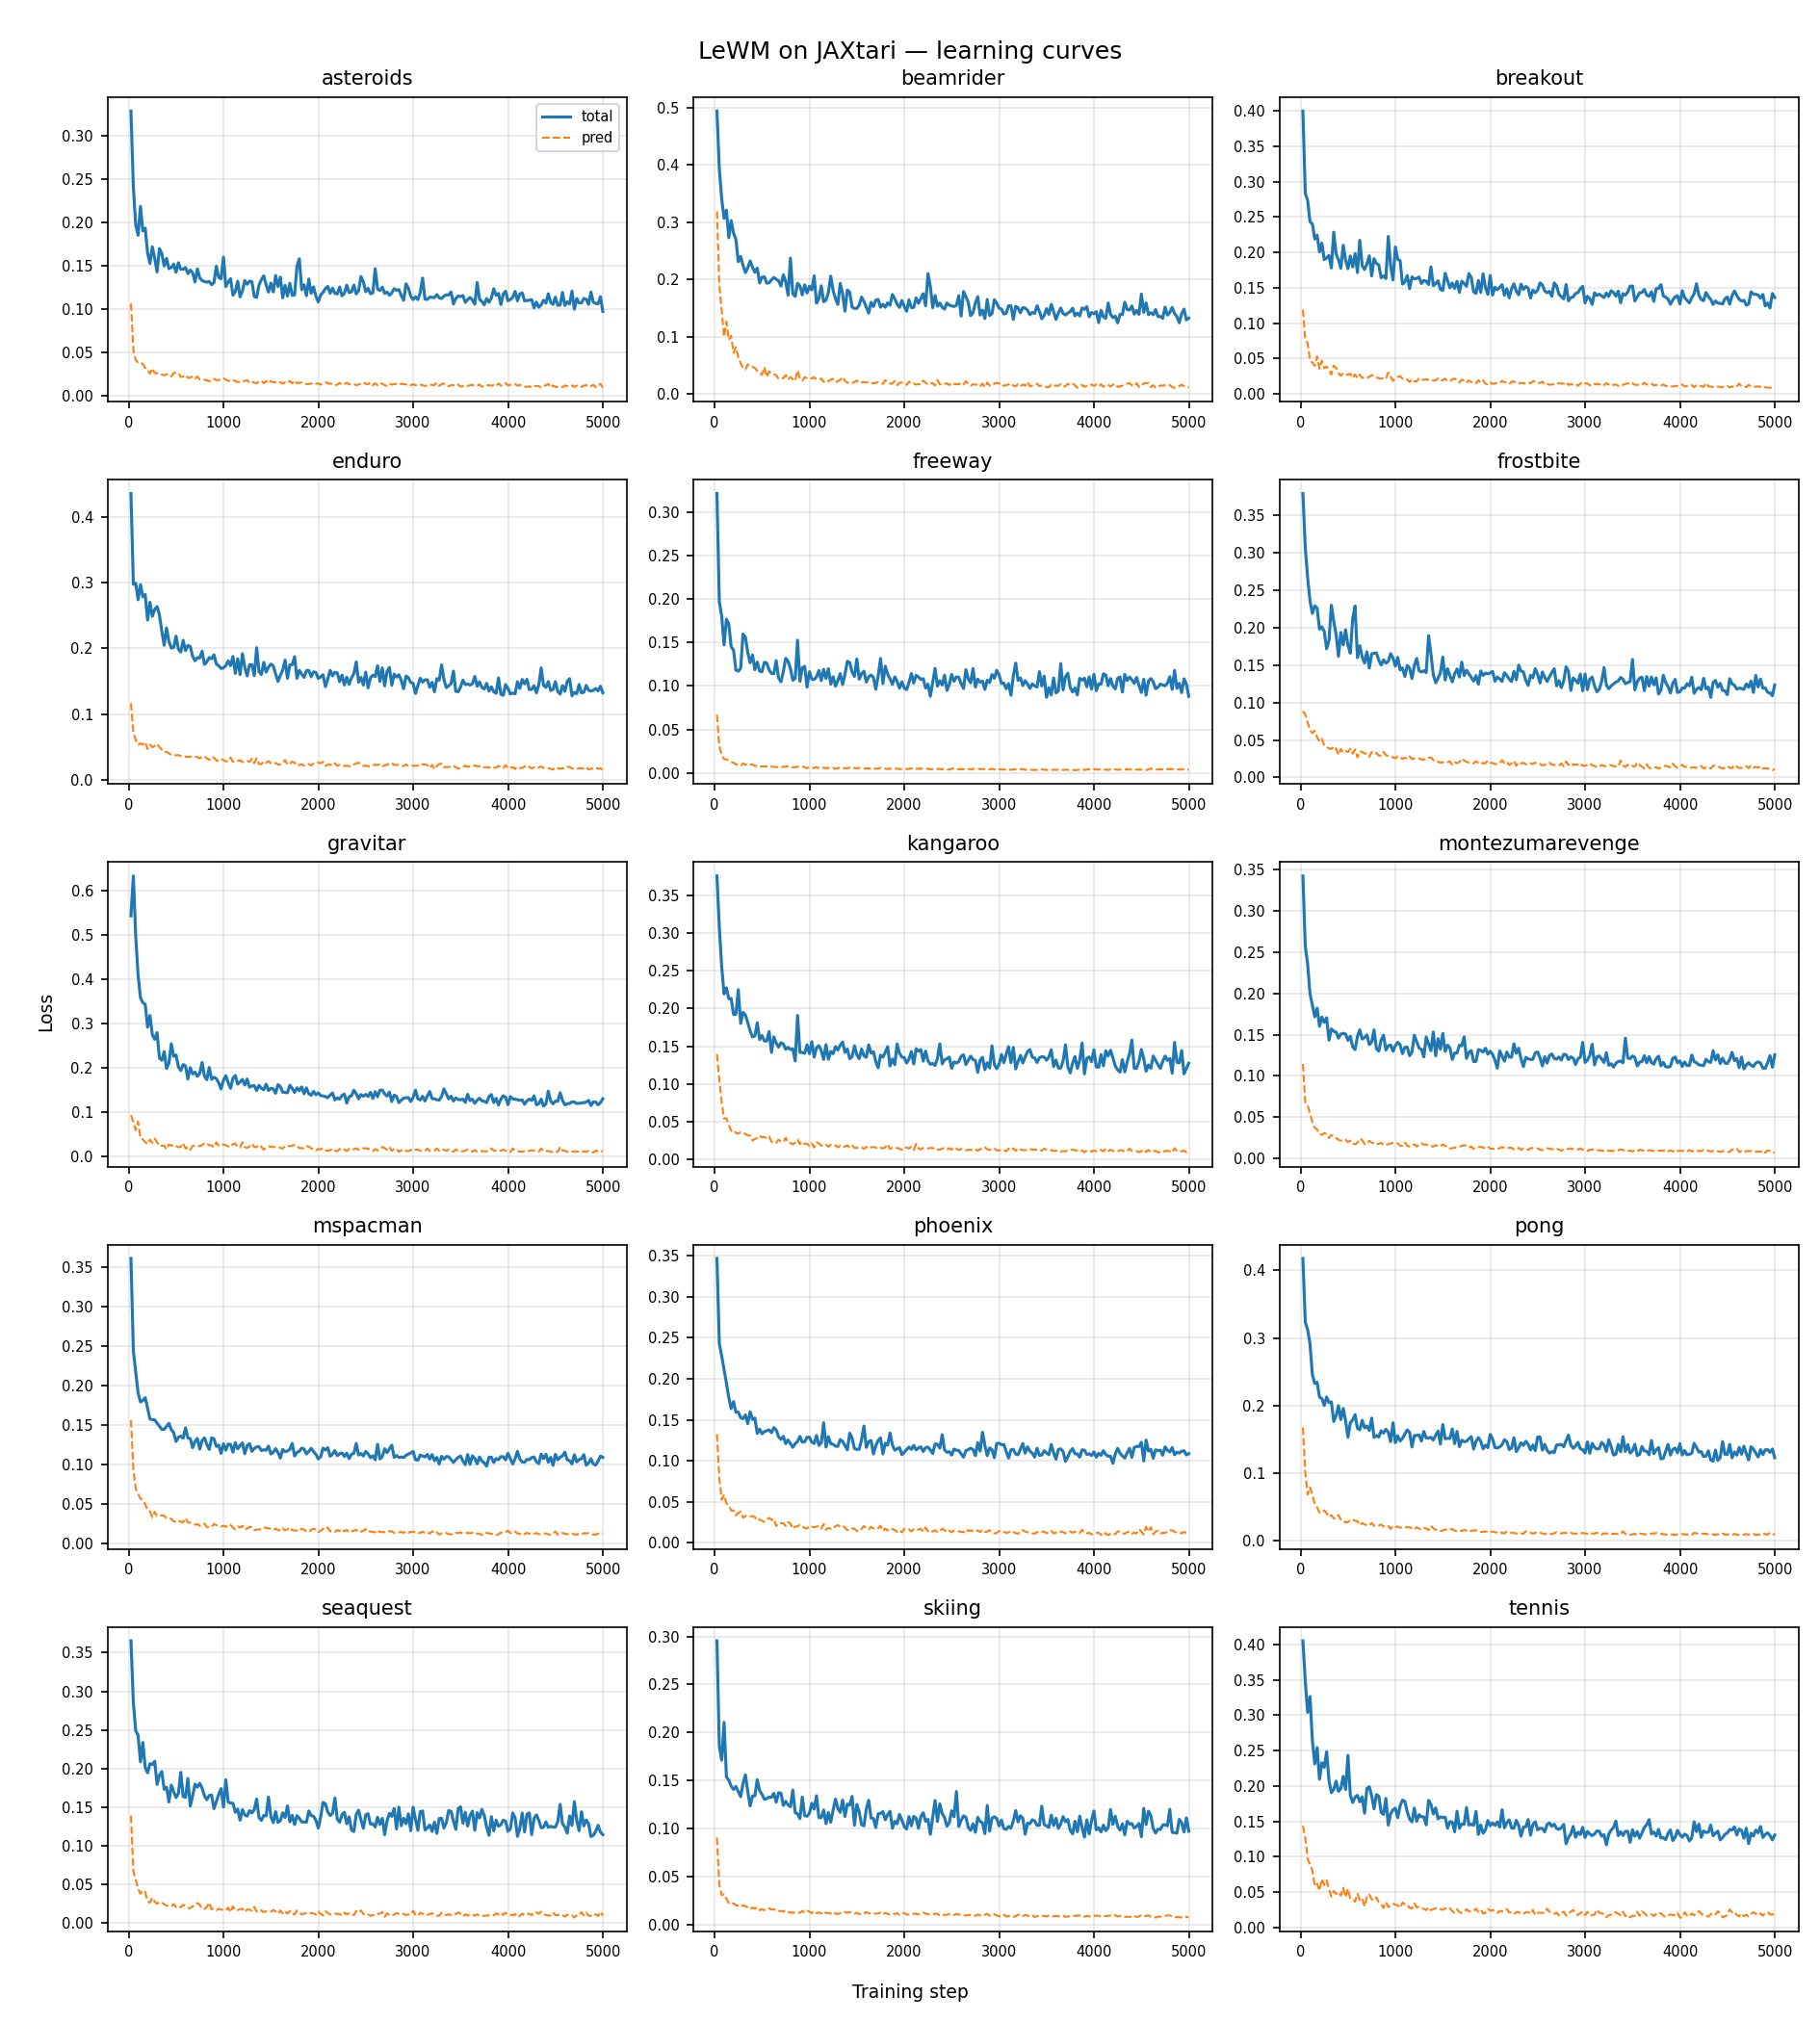
\includegraphics[width=\textwidth]{figures/world_model_curves.png}
\caption{Training curves for all fifteen games. Loss falls smoothly everywhere,
which as argued in Section~\ref{sec:eval} is not by itself evidence that anything
useful was learned.}
\end{figure}

\section{Ablations}
\label{sec:ablations}

The ablations are the most informative part of this work. Each variant changes
exactly one thing relative to the faithful configuration and is trained
identically otherwise, on Pong and on Seaquest.

\begin{table}[h]
\centering
\caption{Ablations after 5000 steps. Values are given as Pong / Seaquest. The
rollout column is the ratio to each variant's own frozen baseline, for the reason
given in Section~\ref{sec:eval}.}
\label{tab:ablations}
\begin{tabular}{lrrr}
\toprule
Variant & Effective rank & Prediction loss & Rollout ratio \\
\midrule
Faithful (the paper)          & 28.4 / 28.5 & \textbf{0.0087 / 0.0113} & \textbf{0.286 / 0.235} \\
No SIGReg ($\lambda = 0$)     & \textbf{1.7 / 1.9} & 0.0010 / 0.0004 & \textbf{1.006} / 0.695 \\
Stop gradient plus SIGReg     & 174.4 / 68.6 & 0.0730 / 0.0526 & 0.379 / 0.356 \\
Stop gradient only            & 149.4 / 42.8 & 0.0960 / 0.0942 & 0.430 / 0.689 \\
Additive action conditioning  & 21.2 / 21.1 & 0.0092 / 0.0115 & 0.310 / 0.188 \\
$\lambda = 0.5$               & 58.9 / 44.6 & 0.0209 / 0.0225 & 0.289 / 0.305 \\
$\lambda = 2.0$               & 89.9 / 59.5 & 0.0399 / 0.0393 & 0.330 / 0.409 \\
\bottomrule
\end{tabular}
\end{table}

\subsection{Removing SIGReg collapses the representation}

With $\lambda = 0$ the effective rank falls to 1.7 on Pong and 1.9 on Seaquest,
which is total collapse. At the same time the prediction loss \emph{improves} by a
factor of nine on Pong and twenty eight on Seaquest, reaching 0.0010 and 0.0004
against 0.0087 and 0.0113 for the faithful configuration.

This is the single most useful result in the report, and not because it is
surprising. It is useful because it makes the failure mode concrete and
quantitative. A practitioner watching only the training loss would conclude that
removing the regulariser had improved the model by an order of magnitude. The
downstream consequence is that on Pong the collapsed model then fails to beat even
its own trivial baseline, at a ratio of 1.006. The model has learned nothing and
the loss curve says it has learned a great deal.

\subsection{The paper's claim, and where it has to be narrowed}

The interesting control is the one with $\lambda = 0$ and a stop gradient enabled,
which is the BYOL style configuration the paper positions itself against. If that
configuration also collapsed, the claim "SIGReg is what prevents collapse" would be
straightforwardly supported.

It does not collapse. Effective rank reaches 149.4 on Pong and 42.8 on Seaquest, in
both cases far from collapse. A plain stop gradient prevents collapse perfectly
well in this setting, without any regulariser at all.

The claim therefore has to be narrowed, and the narrowed version is the one this
report makes. SIGReg is \emph{sufficient} to prevent collapse without a stop
gradient, which is a real and useful property, but it is not \emph{necessary} for
that purpose. What SIGReg contributes over a stop gradient is prediction quality:
its prediction loss is roughly eleven times lower on Pong and eight times lower on
Seaquest than the stop gradient only configuration, and its rollout ratio is better
than either stop gradient variant. Adding a stop gradient on top of SIGReg makes
the model worse rather than better.

A related point is worth stating because it is easy to get backwards. High
effective rank is not itself a goal. The stop gradient variant has the highest rank
of any configuration tested, at 174.4, and a clearly worse rollout ratio than the
faithful configuration. Rank is a diagnostic for collapse, not a measure of
quality.

\subsection{Regularisation strength}

Raising $\lambda$ from 0.1 to 0.5 to 2.0 increases effective rank monotonically and
degrades the rollout ratio monotonically on both games, from 0.286 to 0.289 to
0.330 on Pong and from 0.235 to 0.305 to 0.409 on Seaquest. The value of 0.1
recommended by the paper is therefore also the right value on Atari, which is a
small piece of evidence that the hyperparameter transfers across domains.

\subsection{Action conditioning}

Replacing the adaptive layer normalisation conditioning with a simple additive
action embedding produces essentially no difference. The adaptive scheme gives a
slightly lower prediction loss on both games, while the additive scheme gives a
better rollout ratio on Seaquest and a worse one on Pong.

This result is reported rather than omitted, even though it is unflattering to the
architecture that was implemented faithfully. The honest summary is that the
paper's conditioning mechanism shows no measurable benefit at this scale, and it is
retained in the implementation for fidelity rather than because the evidence
supports it. An earlier version of these experiments had a data bug that corrupted
a quarter of all action labels, described in Section~\ref{sec:confounds}, which
would have been a perfectly good excuse for finding no difference. The numbers
above come from the corrected pipeline and the conclusion did not change.

\begin{figure}[h]
\centering
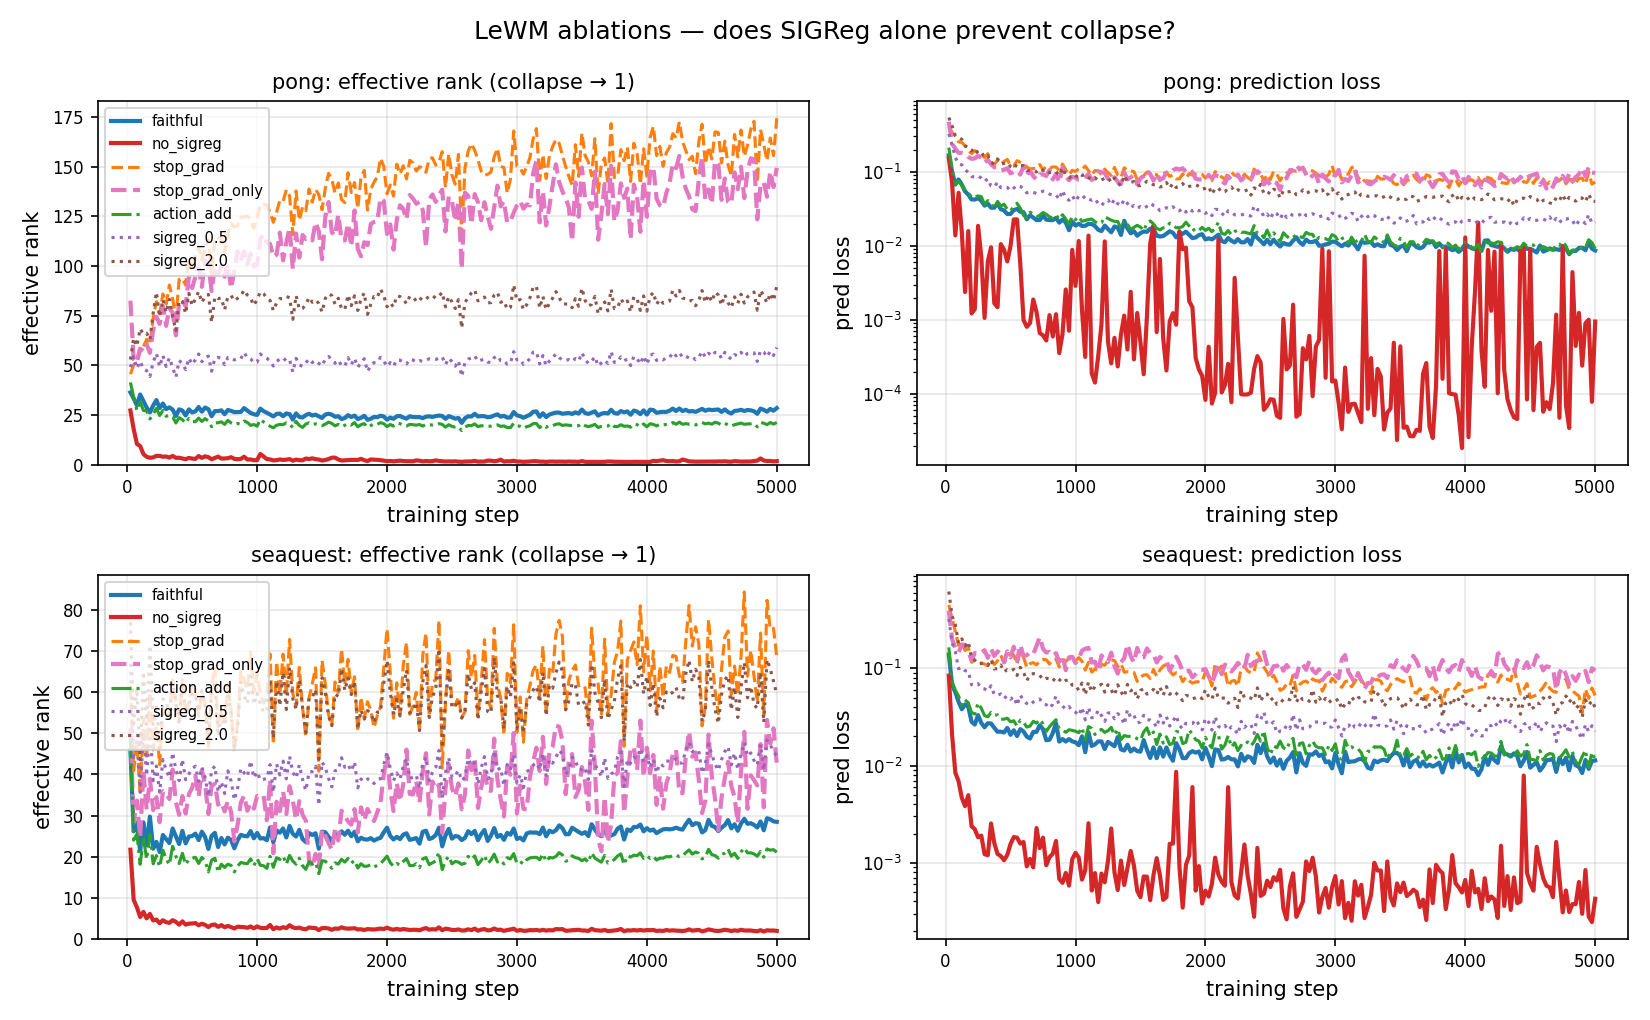
\includegraphics[width=\textwidth]{figures/ablations.png}
\caption{Effective rank and prediction loss over training for every ablation. The
red curve is the configuration without SIGReg. Note that it has both the lowest
rank and the lowest loss, which is the entire point.}
\end{figure}

\section{Downstream evaluation with a reinforcement learning agent}

Because LeWM is trained without rewards, it produces no game scores. To obtain
numbers comparable with published reinforcement learning results, a PPO agent was
trained on top of the learned representation.

\subsection{Setup}

Three configurations share identical policy and value heads, identical
hyperparameters, identical observations and an identical step budget. They differ
in where the features come from:

\begin{itemize}
\item \textbf{scratch}: a Nature CNN trained end to end with the policy. This is the control.
\item \textbf{frozen}: the pretrained LeWM encoder with its weights frozen.
\item \textbf{fine tuned}: the pretrained LeWM encoder, updated by the policy gradient.
\end{itemize}

The world model encodes single frames, so the four frame stack is encoded frame by
frame with the same encoder and the resulting embeddings are concatenated, which is
what gives the policy access to motion.

One caveat about this comparison should be stated plainly, because the natural way
to describe it is too strong. It is not true that the only difference is where the
features come from. The scratch network mixes the four stacked frames
convolutionally and therefore builds spatially local motion features, whereas the
LeWM trunk encodes each frame independently and combines them with a single linear
layer. The two trunks have different access to precisely localised motion, and
that difference is a plausible contributor to the results on Breakout in
particular. It is not controlled for here.

\subsection{Results}

\begin{table}[h]
\centering
\caption{Episodic return after one million environment steps, averaged over the
final ten percent of training. Scores are unclipped game scores. Single seed.}
\label{tab:agents}
\begin{tabular}{lrrr}
\toprule
Game & PPO from scratch & On frozen LeWM & On fine tuned LeWM \\
\midrule
Pong     & 15.3 & \textbf{17.2} & $-15.6$ \\
Seaquest & \textbf{949} & 571 & 411 \\
Breakout & \textbf{40.8} & 12.2 & 12.0 \\
\bottomrule
\end{tabular}
\end{table}

Taken at face value this table suggests that the pretrained representation helps on
Pong and hurts elsewhere. The next section shows that the first half of that
reading does not survive contact with multiple seeds.

\begin{figure}[h]
\centering
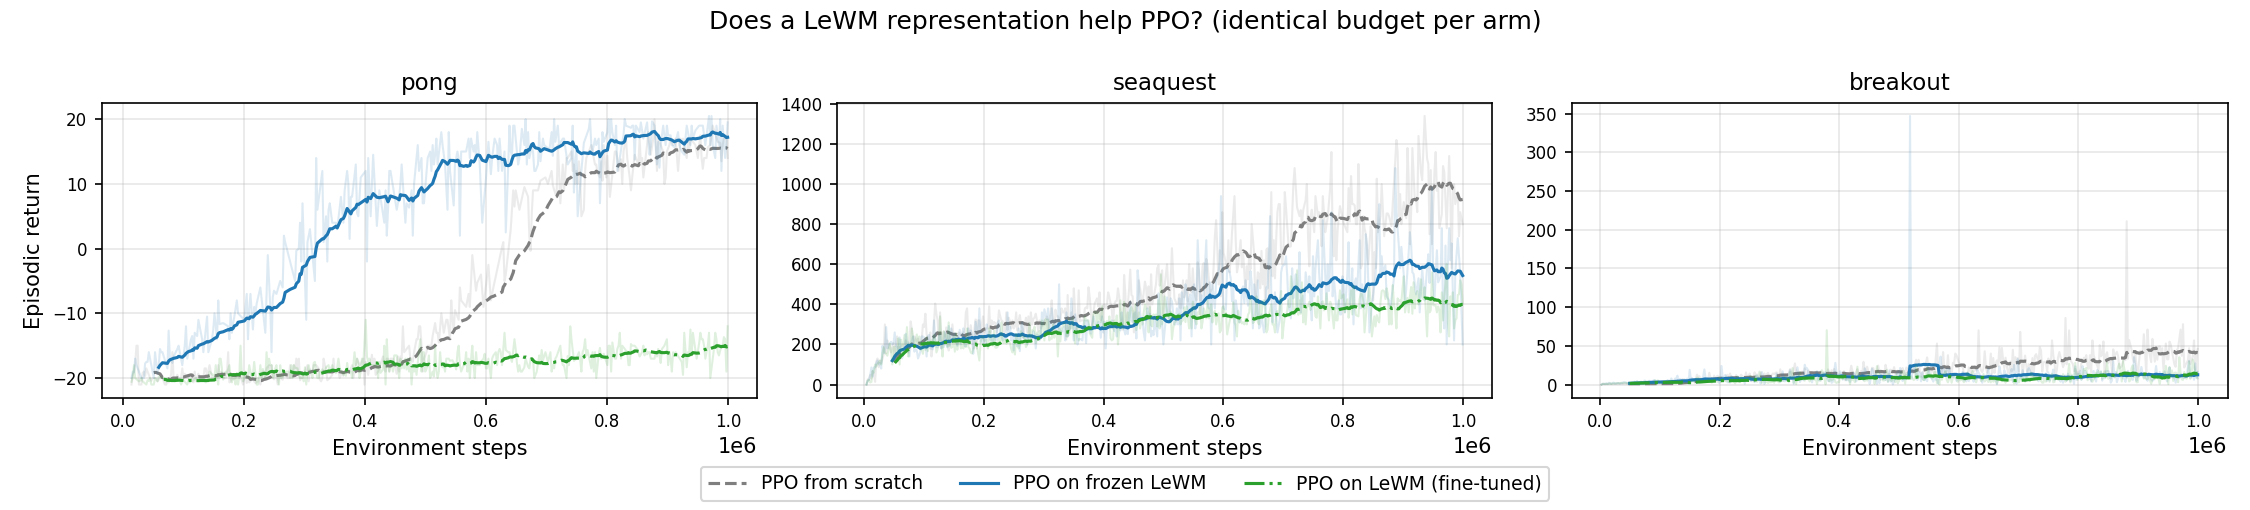
\includegraphics[width=\textwidth]{figures/agent_comparison.png}
\caption{Learning curves for the three configurations on each game, single seed.
The pretrained representation leads early on Pong, tracks the baseline on Seaquest
before falling behind, and plateaus well below it on Breakout.}
\end{figure}

\subsection{Three seeds on Pong}

A single reinforcement learning run on Atari carries very little information, so
Pong was repeated with three seeds.

\begin{table}[h]
\centering
\caption{Pong over three seeds. The two columns measure different things and are
deliberately kept apart.}
\label{tab:seeds}
\begin{tabular}{lrr}
\toprule
 & Final return & Steps to first positive return \\
\midrule
PPO from scratch   & $12.60 \pm 7.27$ & 0.61M \quad [0.63, 0.69, 0.51] \\
PPO on frozen LeWM & $17.36 \pm 1.09$ & \textbf{0.32M} \quad [0.27, 0.40, 0.29] \\
\bottomrule
\end{tabular}
\end{table}

\paragraph{The final score difference is not significant.} The gap between the
means is 4.8 while the standard deviation of the scratch configuration alone is
7.3. A claim that LeWM produces higher final scores on Pong does not survive three
seeds, and no such claim is made in this report. The single seed table above would
have supported exactly that claim, which is a good illustration of why the extra
runs were worth the compute.

\paragraph{Sample efficiency is a clean result.} The number of steps required to
reach positive play is roughly halved, and the per seed values do not overlap at
all. The worst LeWM seed, at 0.40M steps, still reaches positive play sooner than
the best scratch seed at 0.51M. Three out of three. This is the effect that a
pretrained representation is supposed to produce, and unlike the final score it
holds up under repetition.

\paragraph{Variance falls sharply.} The standard deviation drops from 7.27 to 1.09,
roughly a factor of seven. Every LeWM seed lands within a two point band while the
scratch runs span fourteen points. The pretrained representation makes the outcome
of a run predictable as well as faster, which for a practitioner is worth
something on its own.

\begin{figure}[h]
\centering
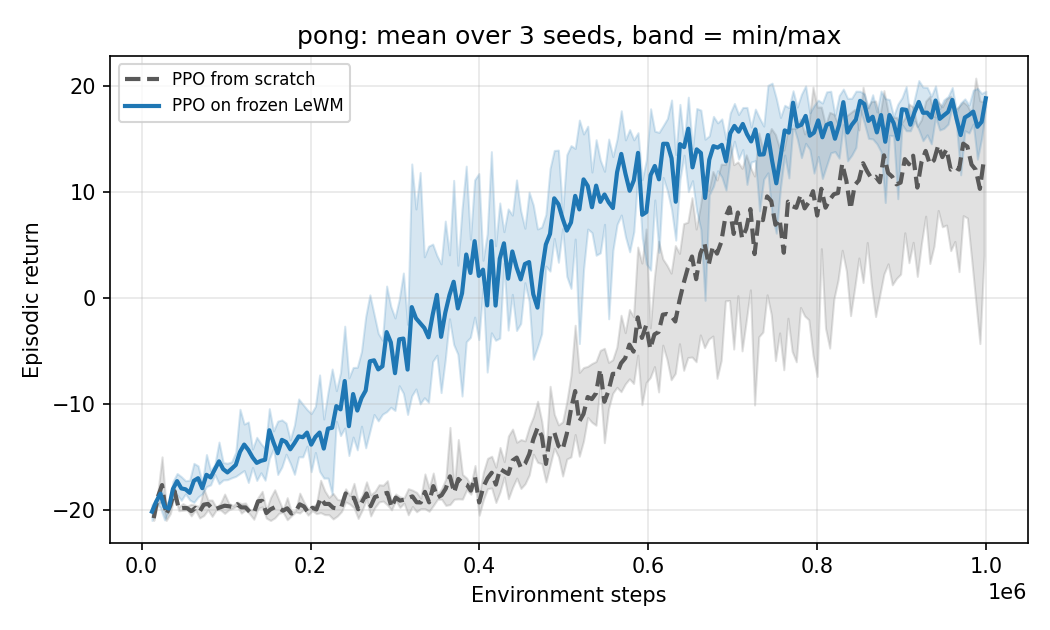
\includegraphics[width=0.85\textwidth]{figures/pong_seeds.png}
\caption{Pong over three seeds. The line is the mean and the band spans the
minimum and maximum over seeds. The two configurations separate early and converge
late, which is the shape a sample efficiency gain has.}
\end{figure}

\subsection{Where the representation does not help}

On Seaquest and Breakout the frozen encoder plateaus clearly below the scratch
network. The obvious explanation is that the encoder was trained on data from a
random policy and therefore goes out of distribution as the policy improves. That
explanation is testable: unfreezing the encoder should allow it to adapt and close
the gap.

It does not. The fine tuned configuration improves Seaquest and Breakout only
marginally, and on Pong it is dramatically worse than leaving the encoder alone.
The distribution shift explanation is therefore not supported by the experiment
designed to test it, and this report does not advance it.

An alternative explanation, which is stated here as a hypothesis and not as a
finding because it has not been tested, is an information bottleneck. LeWM is
optimised to predict, and prediction does not require the information that control
requires. The arrangement of remaining bricks in Breakout barely affects the next
frame but entirely determines the achievable score. Pong may be the exception
precisely because its state essentially is the ball and two paddles, so almost
everything prediction preserves is also what control needs. A linear probe,
measuring how well task relevant quantities can be decoded from the frozen
embedding compared with features from the scratch network, would test this directly
and is the most obvious next experiment.

One further caveat on the fine tuned arm. Pretrained encoder weights are updated at
one tenth of the learning rate used for the freshly initialised heads. At the full
rate training diverges, for reasons explained in Section~\ref{sec:confounds}, while
at the reduced rate the encoder adapts only slightly. Fine tuning here is caught
between instability and inertia, so the result should be read as "does not close
the gap at this setting" rather than as a general statement about fine tuning.

\subsection{Comparison against published scores}

The lab guidelines ask for a comparison against reported PPO scores from the
original ALE implementation. The source they link is the original PPO paper of
Schulman et al. (2017), whose Table 6 reports mean final scores over the last one
hundred episodes after forty million game frames, equivalently ten million
timesteps at a frame skip of four.

\begin{table}[h]
\centering
\caption{This work against the published PPO scores of Schulman et al. (2017),
Table 6. The published column is measured at ten times the step budget used here,
so the columns are not directly comparable and the ratio in the final column is
given to make the size of that gap explicit rather than to hide it.}
\label{tab:published}
\begin{tabular}{lrrrr}
\toprule
Game & Scratch & Frozen LeWM & Published PPO & Ratio \\
     & (1M)    & (1M)        & (10M)         & (best here / published) \\
\midrule
Pong     & 15.3 & 17.2 &   20.7 & 0.83 \\
Seaquest & 949  & 571  & 1204.5 & 0.79 \\
Breakout & 40.8 & 12.2 &  274.8 & 0.15 \\
\bottomrule
\end{tabular}
\end{table}

The budget difference has to be read alongside these numbers. The agents here are
trained for one million environment steps, which is one tenth of the budget behind
the published column, and published Atari results are elsewhere often reported
after two hundred million frames, which is a factor of fifty. Nothing in this table
should be presented as a converged comparison.

With that qualification stated, the pattern is still informative. On Pong and
Seaquest this implementation reaches roughly four fifths of the published score
using one tenth of the interaction, which is the behaviour expected of a correct
implementation stopped early. Breakout is the clear outlier at fifteen percent, and
it is the same game on which the frozen representation performs worst. Breakout
rewards precise tracking of a small fast object, and the limitation noted in
Section~\ref{sec:limitations} applies with particular force there: the LeWM trunk
encodes each frame independently and concatenates the embeddings, so it has weaker
access to precisely localised motion than a network that convolves over the stacked
frames. That this is also the game where the gap to published PPO is widest for
\emph{both} arms suggests the budget is the dominant factor and the representation
a secondary one, but the two are not separated here.

\paragraph{Why this comparison covers scores and not learning curves.} The lab
guidelines ask for a comparison of final scores \emph{and} learning curves against
the original implementations. Only the first is given here, for two reasons that
are worth stating rather than passing over. First, the reference that the
guidelines link publishes a table of final scores and no per game curve data, so
there is no reference curve to plot this work against. Second, and more
fundamentally, LeWM has no score of its own to compare: its reference
implementation is a world model evaluated by planning in the latent space on
different benchmarks, and it never produces a game return. The downstream agent in
this section exists precisely to manufacture a quantity that published
reinforcement learning results can be compared against at all.

A curve level comparison is still possible in principle, by running the
repository's own PPO under an identical budget and overlaying the two curves. That
was attempted and abandoned on time grounds: the repository's PPO is written in
JAX, which has no GPU backend on Apple silicon, and it was measured at roughly
seventeen environment steps per second on the machine in Table~\ref{tab:system},
which puts a single one million step run at about fifteen hours. Increasing the
number of parallel environments from eight to thirty two and then to one hundred
and twenty eight did not improve throughput, so the limit is compute rather than
parallelism. On a CUDA machine this comparison would be inexpensive and it is the
first thing worth adding to this work.

\section{Methodological problems found during the work}
\label{sec:confounds}

Three problems were found and fixed during the project. None of them caused a
crash. All three produced plausible looking numbers that were wrong, which is the
category of bug that is most dangerous in empirical work, so they are documented
here rather than quietly repaired.

\subsection{Corrupted action labels from sticky actions}

The environment wrapper used for world model data collection took its default
setting of a 0.25 sticky action probability, while the wrapper used for the agent
explicitly disabled it. Under stickiness the environment executes the
\emph{previous} action with probability one quarter, but the calling code only ever
sees the action it requested. The world model was therefore learning $p(z' \mid z,
a)$ from action labels that were wrong a quarter of the time.

This directly corrupted the experiment intended to measure action conditioning, and
it also meant the encoder was pretrained under different dynamics than it was
later deployed on. Both environments now disable sticky actions.

\subsection{Coverage restricted to the opening seconds of each game}

Episodes were capped at sixty eight environment steps, and the windows kept from
each episode were taken from the front. The model therefore never observed any part
of a game beyond roughly the first four and a half seconds of play.

Investigating this revealed a second cause that was easy to miss. On games with
short lives the cap was not even the binding constraint. With episodic life
handling enabled, an episode ends at the first lost life, which under a random
policy is about twenty two steps in Breakout. The model could not have seen a
partly cleared brick wall regardless of the cap.

Both were fixed. Episodic life handling is disabled for reward free collection,
where it serves no purpose, episodes now run up to five hundred steps, and windows
are sampled across the whole episode. Measured effect: Breakout episodes went from
twenty two steps to two hundred and seventeen, Pong and Seaquest from sixty eight
to five hundred and four hundred and thirty four.

This matters for interpretation and not only for tidiness. A model that has never
seen a partly cleared brick wall has a coverage based explanation for its poor
Breakout performance, and that explanation was confounded with the information
bottleneck hypothesis discussed above.

\subsection{Batch normalisation inside a PPO policy trunk}

When the encoder was fine tuned it remained in training mode, so its batch
normalisation layers normalised using batch statistics during the policy update but
running statistics during the rollout, with batch sizes differing by a factor of
thirty two between the two.

This interacts badly with PPO specifically. PPO stores action log probabilities
during the rollout and recomputes them during the update in order to form an
importance ratio. If the two passes are computed by functions that differ, the
ratio is meaningless. Training diverged, with the value loss reaching $10^{15}$ and
the policy entropy collapsing to zero within twenty five iterations on every game.

The fix is to keep the encoder's normalisation layers in inference mode at all
times, so that only the weights are updated. This removed the divergence but
introduced the second problem noted earlier: with the normalisation statistics
fixed, nothing constrains the scale of the encoder's output, and at the full
learning rate the embeddings drift until the policy logits saturate. Hence the
reduced learning rate for pretrained weights. The general lesson, which
generalises beyond this project, is that batch normalisation inside a policy trunk
is specifically hazardous for algorithms that compare two forward passes.

\section{Limitations}
\label{sec:limitations}

\begin{itemize}

\item \textbf{Compute budget.} Agents are trained for one million environment steps
against a reference of two hundred million. The curves show learning trends and not
converged performance.

\item \textbf{Seeds.} Pong uses three seeds. Every other agent number in this
report comes from a single seed and should be read as indicative only. The Pong
result demonstrates why this matters, since one claim survived the addition of
seeds and another did not.

\item \textbf{The agent comparison is not purely a comparison of features}, for the
architectural reason given above.

\item \textbf{Random collection policy.} The world model observes only the states a
random agent reaches, which is a small part of the state space on sparse reward
games.

\item \textbf{Evaluation detail.} The rollout evaluation keeps batch normalisation
in batch statistics mode for consistency with training. Using fixed running
statistics instead changes the rollout error by about seven percent, measured on
Pong. That figure is the size of the methodological uncertainty underneath the
rollout numbers in this report.

\item \textbf{Ms.\ Pacman fails} the rollout evaluation and this is not explained.

\item \textbf{The predictor is never used for control}, which is the paper's own
evaluation method.

\end{itemize}

\section{Conclusion}

LeWorldModel was implemented from scratch for JAXAtari and trains stably across the
full fifteen game suite without representation collapse, producing useful open loop
latent predictions on fourteen of the fifteen games.

The ablations support a narrowed version of the paper's central claim. Removing
SIGReg collapses the representation completely while improving the training loss by
up to a factor of twenty eight, which makes the point that this objective cannot be
monitored through its loss. However, a plain stop gradient also prevents collapse,
so SIGReg is sufficient rather than necessary for that purpose. Its actual
contribution is prediction quality, where it beats the stop gradient configurations
by roughly an order of magnitude.

Downstream, the pretrained representation roughly halves the environment steps
needed to reach positive play on Pong, with no overlap across three seeds, and
reduces run to run variance by a factor of about seven. It does not produce a
significantly higher final score, and on Seaquest and Breakout it plateaus below an
equivalent agent trained from pixels. Fine tuning does not close that gap, which
rules out the most obvious explanation and leaves an open question.

The most valuable extensions, in order, would be latent model predictive control so
that the predictor is evaluated the way the paper intends, a linear probe to test
the information bottleneck hypothesis, and additional seeds on the remaining games.

\section*{Code and reproducibility}

The implementation lives in \texttt{scripts/benchmarks/jepa/} in the JAXAtari
repository. The world model is a single self contained file. Eighteen unit tests
cover the properties that fail silently rather than loudly, including the collapse
diagnostic, predictor causality, and two regression tests for bugs described in
Section~\ref{sec:confounds}. Every experiment in this report can be reproduced with
the commands documented in the accompanying README, with a fixed seed.

\section*{Use of AI assistance}

Claude (Anthropic) was used throughout the implementation and analysis, in line
with the course's stated position on the use of language models. It contributed to
writing and debugging code, to designing the evaluation protocol, and to drafting
this report. All experiments were run and inspected by the author, and the numbers
reported here come from the recorded output of those runs. Three of the corrections
described in Section~\ref{sec:confounds} were identified during review of the
generated code rather than at the time of writing, which is itself a reason to
treat generated experimental code with the same suspicion as any other.

\section*{References}

\begin{enumerate}
\item Maes, Le Lidec, Scieur, LeCun and Balestriero. \emph{LeWorldModel: Stable End
to End Joint Embedding Predictive Architecture from Pixels}. arXiv:2603.19312,
2026. Reference implementation: \url{https://github.com/lucas-maes/le-wm}
\item Schulman, Wolski, Dhariwal, Radford and Klimov. \emph{Proximal Policy
Optimization Algorithms}. arXiv:1707.06347, 2017.
\item Huang et al. \emph{CleanRL: High quality single file implementations of deep
reinforcement learning algorithms}. The PPO implementation here follows the
repository's adaptation of CleanRL.
\item Delfosse et al. JAXAtari. \url{https://github.com/k4ntz/JAXAtari}
\end{enumerate}

\end{document}
